% Asset ID: A21TrigonometricFunctionsTikZ-002
% Source: Chapter 6 Trigonometric Functions notation warning + CCEA A21-TRIG-LO002
% Related lesson section: Key Definitions and Notation
% Purpose: Show that cos^{-1}(x) means arccos(x), not 1/cos(x).

\documentclass[tikz,border=8pt]{standalone}
\usepackage{amsmath}
\usetikzlibrary{positioning, arrows.meta}
\begin{document}
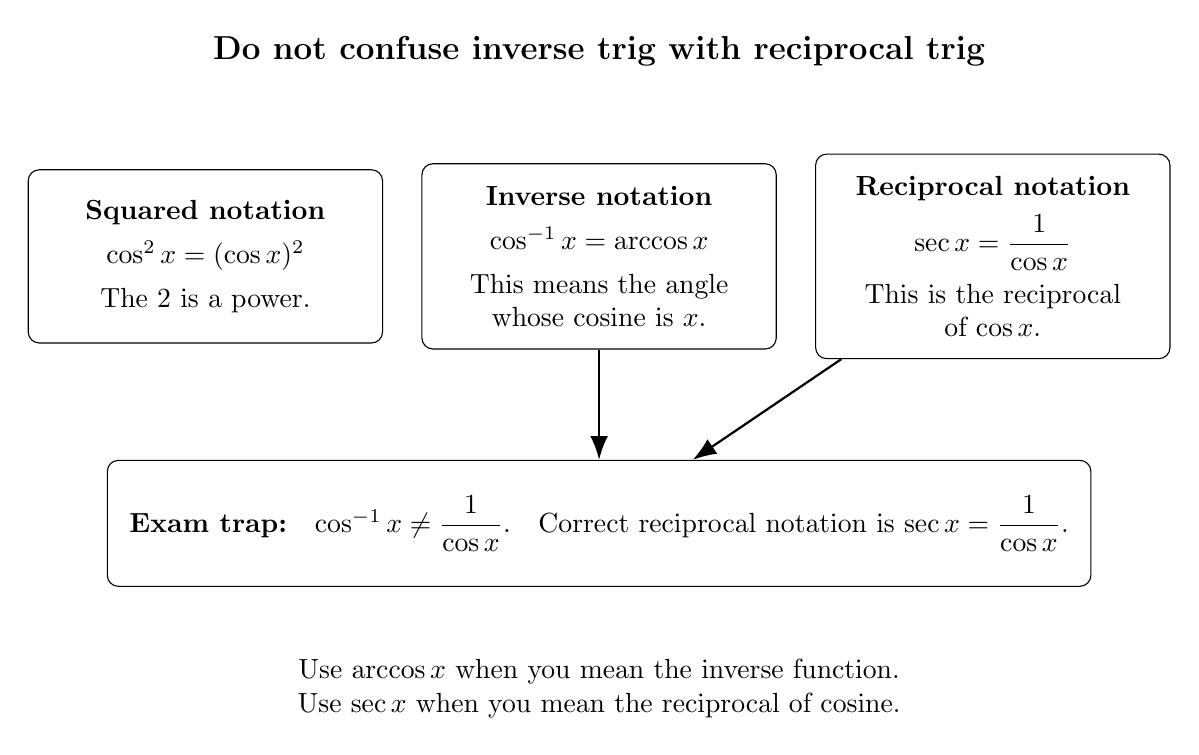
\begin{tikzpicture}[box/.style={draw,rounded corners,align=center,minimum width=4.5cm,minimum height=2.2cm,inner sep=8pt},warning/.style={draw,rounded corners,align=center,minimum width=10cm,minimum height=1.6cm,inner sep=8pt},arrow/.style={-{Latex[length=3mm]},thick},heading/.style={font=\large\bfseries}]
\node[heading] at (0,2.6) {Do not confuse inverse trig with reciprocal trig};
\node[box] (squared) at (-5,0){\textbf{Squared notation}\\[4pt]$\cos^2 x=(\cos x)^2$\\[4pt]The $2$ is a power.};
\node[box] (inverse) at (0,0){\textbf{Inverse notation}\\[4pt]$\cos^{-1}x=\arccos x$\\[4pt]This means the angle\\whose cosine is $x$.};
\node[box] (reciprocal) at (5,0){\textbf{Reciprocal notation}\\[4pt]$\sec x=\dfrac{1}{\cos x}$\\[4pt]This is the reciprocal\\of $\cos x$.};
\node[warning, below=1.4cm of inverse] (bad){\textbf{Exam trap:}\quad $\cos^{-1}x\ne\dfrac{1}{\cos x}$.\quad Correct reciprocal notation is $\sec x=\dfrac{1}{\cos x}$.};
\draw[arrow] (inverse) -- (bad);\draw[arrow] (reciprocal) -- (bad);
\node[below=0.8cm of bad, align=center] {Use $\arccos x$ when you mean the inverse function.\\Use $\sec x$ when you mean the reciprocal of cosine.};
\end{tikzpicture}
\end{document}
